\documentclass[12pt,letterpaper]{article}
\usepackage{amsmath,amssymb,xfrac}
\usepackage[margin=1in]{geometry}
\usepackage{fancyhdr}
\usepackage[utf8]{inputenc}
\usepackage{palatino}
\usepackage{microtype}
\usepackage{hyperref}
\usepackage{graphicx}
\usepackage{lastpage}
\usepackage[hang,small,margin=1in]{caption}
\usepackage{titlesec}

\renewcommand{\headrulewidth}{0pt}
\fancyfoot{}
\fancyfoot[C]{\sffamily Page \thepage\ of~\pageref{LastPage}}
\pagestyle{fancy}

\titleformat{\section}{\bfseries\MakeUppercase}{\arabic{\thesection}}{1em}{}
\titleformat{\subsection}{\bfseries}{\arabic{\thesection}.\arabic{\thesubsection}}{1em}{}
\titleformat{\subsubsection}{\itshape}{\arabic{\thesection}.\arabic{\thesubsection}.\arabic{\thesubsubsection}}{1em}{}

\setlength{\parindent}{0cm}
\setlength{\parskip}{1em}

\captionsetup[figure]{labelfont=it, font=it}
\captionsetup[table]{labelfont={it,sc}, font={it,sc}}

\hypersetup{colorlinks, linkcolor = black, citecolor = black, urlcolor = black}
\urlstyle{same}



\begin{document}

\fancyfoot{}
\begin{center}
  \hfill \\
  \vspace{4in}
  {\bf\Huge MTH351 Assignment 5} \\
  \vspace{2in}
  {\Large Soo-Hyun Yoo \\ 930569466 \\ May 27, 2015}
\end{center}

\newpage
\fancyfoot[C]{\sffamily Page \thepage\ of~\pageref{LastPage}}

% Use notes from weeks 7 and 8

\begin{enumerate}
  \item
    \begin{enumerate}
      \item
        \begin{align*}
          \begin{bmatrix}
            1 & 1 & 1 \\
            1 & 2 & 4 \\
            1 & 3 & 9
          \end{bmatrix}
          \begin{bmatrix}
            a_0 \\ a_1 \\ a_2
          \end{bmatrix}
          &=
          \begin{bmatrix}
            1 \\ 2 \\ 6
          \end{bmatrix}
        \end{align*}
        Using Matlab to solve for the coefficients, we get \[P_2(x)=\frac32x^2-\frac72x+3.\]
        % syms a0 a1 a2
        % a=[1,1,1;1,2,4;1,3,9]; b=[1;2;6]
        % [r0,r1,r2] = solve(a*[a0;a1;a2]==b)

      \item We have
        \begin{align*}
          L_0(x) &= \frac{(x-2)(x-3)}{(1-2)(1-3)} \\
                 &= \frac12(x-2)(x-3) \\
          L_1(x) &= \frac{(x-1)(x-3)}{(2-1)(2-3)} \cdot 2 \\
                 &= -2(x-1)(x-3) \\
          L_2(x) &= \frac{(x-1)(x-2)}{(3-1)(3-2)} \cdot 6 \\
                 &= 3(x-1)(x-2),
        \end{align*}
        so
        \begin{align*}
          P_2(x) &= L_0(x) + L_1(x) + L_2(x) \\
                 &= \frac12(x-2)(x-3) - 2(x-1)(x-3) + 3(x-1)(x-2) \\
                 &= \frac12(x^2-5x+6) - 2(x^2-4x+3) + 3(x^2-3x+2) \\
                 &= \left(\frac12-2+3\right)x^2 + \left(-\frac52+8-9\right)x + (3-6+6) \\
                 &= \frac32x^2 - \frac72x + 3,
        \end{align*}
        as desired.

      \item The table of Newton's divided differences is as follows:
        \begin{align*}
          \begin{matrix}
            1 & 1 \\
            2 & 2 & \frac{2-1}{2-1}=1 \\
            3 & 6 & \frac{6-2}{3-2}=4 & \frac{4-1}{3-1}=\frac32
          \end{matrix}
        \end{align*}
        So
        \begin{align*}
          P_2(x) &= 1 + 1(x-1) + \frac32(x-1)(x-2) \\
                 &= 1 + x - 1 + \frac32x^2 - \frac92x + 3 \\
                 &= \frac32x^2 - \frac72x + 3. \quad \checkmark
        \end{align*}
    \end{enumerate}

  \item
    \begin{enumerate}
      \item The upper bound on the error in the interpolating polynomial
        \[f(x^*) - P_4(x^*)
        = \frac{f^{(n+1)}(\xi_{x^*})}{(n+1)!}\prod_{i=0}^n(x^*-x_i).\]

      \item If the interpolating nodes are equally spaced at $x=\{0,1,2,3,4\}$,
        then
        \[f^5(x) \leq \left(\frac\pi2\right)^5\cos\left(\frac\pi2x\right),\]
        which is maximized at $\left(\frac\pi2\right)^5$ when cos is 1. So, the
        error at $x^*=\frac12$ should be less than
        \[\frac{\left(\frac\pi2\right)^5}{5!}
          \left(\frac12\right)
          \left(-\frac12\right)
          \left(-\frac32\right)
          \left(-\frac52\right)
          \left(-\frac72\right)
        \approx 0.261491.\]
        Using {\tt lagrange\_interp.m}, we find the error of the polynomial
        approximation at $x^*=\frac12$ is $\sin\left(\frac\pi4\right)-0.875
        = \boxed{0.167893} < 0.261491. \quad \checkmark$

      \item Using the five Chebyshev interpolation points $x=\{0.0979, 0.824,
        2.00, 3.18, 3.90\}$, we find the error at $x^*=\frac12$ is only
        $0.0909259$, which is less than with equally spaced points.

      \item Although the Chebyshev interpolation is a better fit overall, the
        interpolation on the equally spaced $x$ values is closer to the
        original function near $x=2$, the center of the range.
        \begin{figure}[!h]
          \centering
          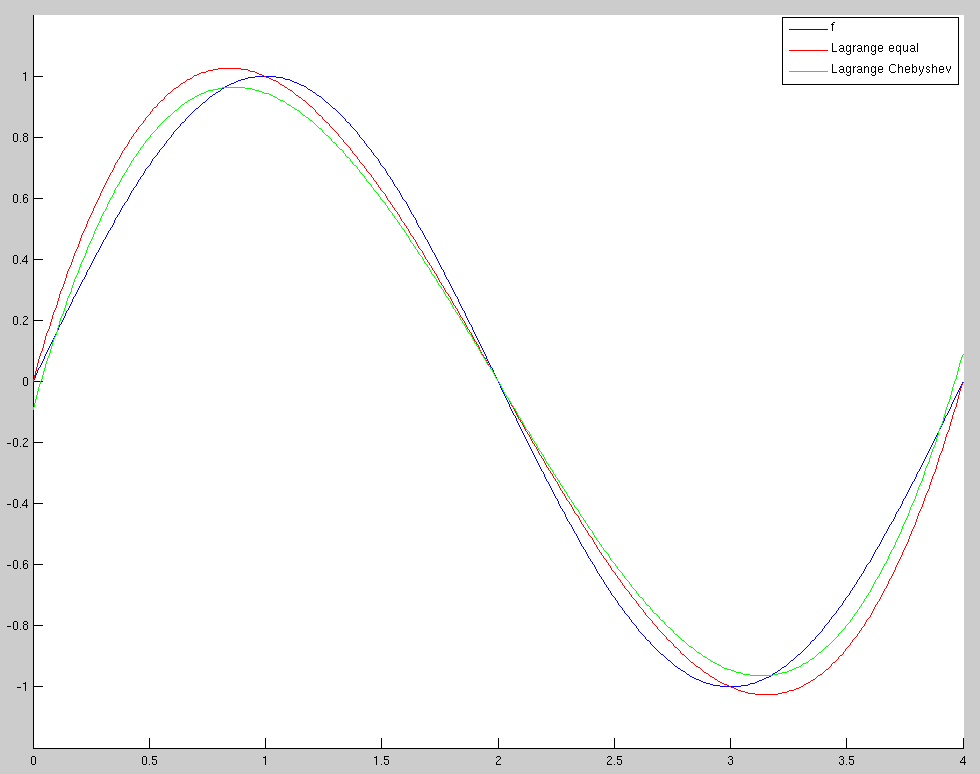
\includegraphics[width=0.8\textwidth]{img/2d.png}
        \end{figure}
    \end{enumerate}

  \item
    \begin{enumerate}
      \item Given the table
        \begin{align*}
          \begin{matrix}
            0 & 0 \\
            0 & 0 & 1 \\
            1 & 1 & \frac{1-0}{1-0}=1 & \frac{1-1}{1-0}=0 \\
            1 & 1 & 0 & \frac{0-1}{1-0}=-1 & \frac{-1-0}{1-0}=-1,
          \end{matrix}
        \end{align*}
        \begin{enumerate}
          \item The Lagrange interpolant of degree 1 is
            \[P_1(x) = 0 + 1(x-0) = x.\]
          \item The Hermite interpolant of degree 3 is
          \begin{align*}
            H_3(x) &= 0 + 1(x-0) + 0(x-0)^2 - 1(x-0)^2(x-1) \\
                   &= -x^3 + x^2 + x.
          \end{align*}
        \end{enumerate}

      \item Both $P_1$ and $H_3$ hit the data points 0 and 1, but $H_3$ stays
        much closer to $f$ than $P_1$ between 0 and 1 (and a bit beyond).
        \begin{figure}[!h]
          \centering
          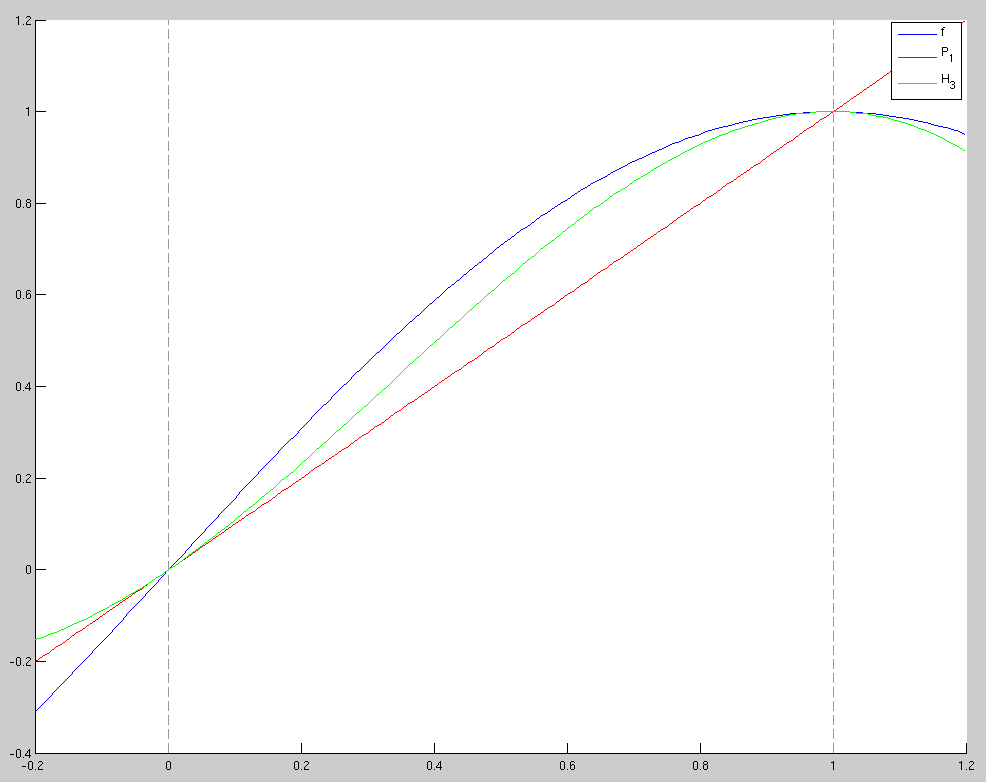
\includegraphics[width=0.8\textwidth]{img/3b.png}
        \end{figure}

      \item The Lagrange interpolant for $n+1$ points of data is a polynomial
        of degree $n$. The Hermite interpolant for the same number of data
        points does not share the same degree. Polynomial approximations of
        higher degrees than $n$ exist for $n+1$ points, but the proof of
        uniqueness was for the lowest-degree Lagrange interpolant only. The
        existence of a Hermite interpolant of degree $2n+1$ does not contradict
        this theorem.
    \end{enumerate}
\end{enumerate}

\end{document}
